\subsection{Workbench}\label{workbench}
De workbench biedt een handig overzicht voor (eind)redacteuren. Via de workbench kun je bijvoorbeeld makkelijk bekijken welke inhoud recentelijk is aangemaakt of welke inhoud nog beoordeeld moet worden.

\subsubsection{Workbench overview}\label{workbenchoverview}
De onderstaande screenshot toont de Workbench. 
\bigskip

\begin{center}
	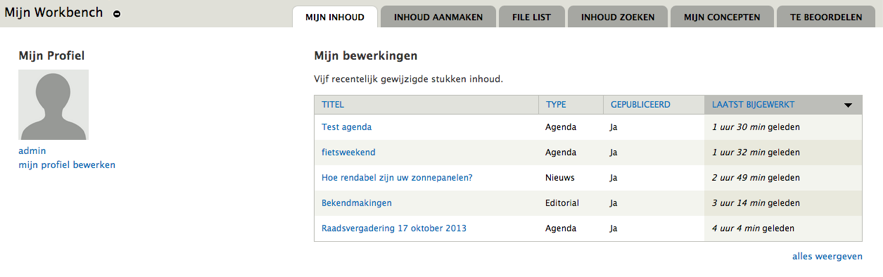
\includegraphics[width=\textwidth]{img/workbench.png}
\end{center}

\textbf{Mijn inhoud:} toont de inhoud welke recentelijk is bewerkt door de gebruiker .

\textbf{Inhoud toevoegen:} link naar de pagina 'Inhoud toevoegen'.

\textbf{File list:} toont alle bestanden welke recentelijk zijn toegevoegd.

\textbf{Inhoud zoeken:} link naar de pagina 'Inhoud zoeken', hier kun je gemakkelijk met behulp van filters op inhoud zoeken.

\textbf{Mijn concepten:} toont alle concepten aangemaakt door de gebruiker 

\textbf{Te beoordelen:} toont alle content items welke nog goedgekeurd moeten worden door de eindredacteur.

\subsubsection{Workbench workflow}\label{workbenchworkflow}
workbench workflow

aanvullen a.u.b. 